\documentclass[a4paper, 12pt]{book}
\usepackage[margin=2.5cm]{geometry}
\usepackage[italian]{babel}
%\usepackage{wrapfig}
\usepackage{graphicx}
\usepackage{hyperref}
\usepackage{amsthm}       % per \theoremstyle e ambienti tipo theorem, definition, example
\usepackage{mdframed}     % per \newmdtheoremenv (ambienti incorniciati)
\usepackage{float}
\usepackage{mdframed}
\usepackage{listings}
\usepackage{amsmath}
\setlength{\parindent}{0pt}
\usepackage{parskip}
\usepackage[most]{tcolorbox}
\usepackage{amsfonts}
\usepackage{}
\usepackage{amssymb}
\usepackage{soul}
\usepackage{xcolor}
\usepackage{amsmath}
\sethlcolor{yellow}
\usepackage{array}
\usepackage{booktabs}
\usepackage{tikz}
\usetikzlibrary{positioning}
\usepackage{longtable}
\usepackage{array}
\usepackage{fancyhdr}
\setlength{\headheight}{15pt}
\pagestyle{fancy}
\fancyhf{} % pulisce header e footer
\fancyhead[R]{\thepage} % numero pagina a destra nell'header
\renewcommand{\headrulewidth}{0pt} % (opzionale) elimina la riga orizzontale sotto l'header
\fancypagestyle{plain}{%
  \fancyhf{} % pulisce header e footer
  \fancyhead[R]{\thepage} % numero sempre in alto a destra
  \renewcommand{\headrulewidth}{0pt} % opzionale: niente linea
}
\setcounter{tocdepth}{3}

\title{\textbf{Intelligenza artificiale}}
\author{Mattia Nicolis}
\date{A.A. 2025-26}

\begin{document}

    \maketitle

    \tableofcontents
    \markboth{}{}

    %-------MODULO DI TEORIA------------------------------------
    %-------Prof: Alessandro Farinell---------------------------
    %-------Lez: mercoledì (8:30-11:30) [Aula Delta - Cav.3]----
    %-------Libro: Artificial Intelligence: a modern approach---



    % Example frame
    \newmdenv[
      linecolor=gray,
      backgroundcolor=gray!10,
      innertopmargin=8pt,
      innerbottommargin=8pt
    ]{example}




    \chapter*{Introduzione all'intelligenza artificiale}
    \addcontentsline{toc}{chapter}{Introduzione all'intelligenza artificiale}
    Il \hl{compito dell’\textbf{intelligenza artificiale} (IA) non è solo quello di \textit{comprendere}, ma anche di \textit{costruire} entità intelligenti}: macchine in grado di calcolare come agire in modo efficace e sicuro in un’ampia varietà di situazioni nuove.

    In passato, gli studiosi hanno proposto diverse versioni di IA: alcuni hanno definito l’intelligenza in termini di fedeltà alla \textbf{prestazione umana}, mentre altri preferiscono una definizione formale di intelligenza come \textbf{razionalità}.

    I metodi utilizzati sono necessariamente diversi: l’approccio che persegue un’intelligenza simile a quella umana deve essere in parte una scienza empirica correlata alla psicologia, richiedendo osservazioni e ipotesi riguardo al comportamento umano e ai processi di pensiero.

    Un approccio razionalista, invece, sfrutta una combinazione di matematica e ingegneria e si collega alla statistica, alla teoria del controllo e all’economia.

    \begin{tcolorbox}[
      colback=cyan!5!white,
      colframe=blue!50!black,
      title=\textbf{Test di Turing},
      coltitle=white,
      fonttitle=\bfseries,
      arc=3mm,
      boxrule=0.5pt,
      enhanced,
      breakable
    ]
      Il \textbf{test di Turing}, proposto da Alan Turing nel 1950, mira a comprendere se una macchina è in grado di pensare.

      \vspace{2mm}

      Un computer supera il test se un esaminatore umano, dopo aver posto alcune domande in forma scritta, non è in grado di distinguere se le risposte provengano da una persona o da una macchina.

      \vspace{2mm}

      Per superare il test, il computer deve possedere le seguenti capacità:
      \begin{itemize}
        \item \textbf{interpretazione del linguaggio naturale}, per comunicare con successo nel linguaggio umano
        \item \textbf{rappresentazione della conoscenza}, per memorizzare ciò che conosce o apprende
        \item \textbf{\textbf{ragionamento automatico}}, per rispondere alle domande e trarre nuove conclusioni
        \item \textbf{apprendimento automatico} (\textit{machine learning}), per adattarsi a nuove circostanze, individuare ed estrapolare schemi
      \end{itemize}

      \vspace{2mm}

      Esiste, inoltre, un cosiddetto \textbf{test di Turing totale}, che richiede l’interazione con oggetti e persone nel mondo reale.

      \vspace{2mm}

      Per superare il test di Turing totale, un robot deve anche possedere:
      \begin{itemize}
        \item \textbf{visione artificiale} e riconosciemtno vocale, per percepire il mondo
        \item \textbf{robotica}, per manipolare gli oggetti e muoversi fisicamente
      \end{itemize}
    \end{tcolorbox}

    \section*{Tipologie di intelligenza artificiale}
    \addcontentsline{toc}{section}{Tipologie di intelligenza artificiale}

    \subsection*{\textcolor{blue}{Agenti autonomi}}
    \addcontentsline{toc}{subsection}{Agenti autonomi}
    Sono sistemi che percepiscono l’ambiente e agiscono in modo autonomo per raggiungere obiettivi specifici.

    \subsection*{\textcolor{blue}{Data analysis}}
    \addcontentsline{toc}{subsection}{Data analysis}
    Consiste nell’utilizzo di algoritmi per analizzare grandi quantità di dati ed estrarre informazioni utili e correlazioni complesse.

    \subsection*{\textcolor{blue}{Machine Learning}}
    \addcontentsline{toc}{subsection}{Machine Learning}
    È lo sviluppo di algoritmi che permettono ai modelli di apprendere dai dati di esempio e migliorare le proprie prestazioni nel tempo, senza essere esplicitamente programmati.
    
    Un esempio è il riconoscimento di immagini.

    L’apprendimento automatico si divide in tre categorie principali:
    \begin{itemize}
      \item \textbf{unsupervised learning}: l modello viene addestrato su dati non etichettati, con l’obiettivo di scoprire strutture nascoste o pattern nei dati senza risposte predefinite.
    \item \textbf{supervised learning}: l modello viene addestrato su dati etichettati, dove ogni input è associato a una risposta corretta. L’obiettivo è imparare a mappare correttamente gli input alle risposte
      \item \textbf{reinforced learning}: il modello apprende attraverso interazioni con l’ambiente, ricevendo ricompense o penalità in base alle azioni compiute. L’obiettivo è massimizzare la ricompensa totale nel tempo
    \end{itemize}

    \subsection*{\textcolor{blue}{Time series analysis}}
    \addcontentsline{toc}{subsection}{Time series analysis}
    L’analisi delle serie temporali è un’area dell’apprendimento automatico che si concentra sull’analisi di dati raccolti nel tempo.

    Le serie temporali sono sequenze di dati misurati a intervalli regolari, come la temperatura giornaliera, i prezzi delle azioni o i dati di vendita mensili.

    L’obiettivo è identificare pattern, tendenze e stagionalità per effettuare previsioni future.

    \vspace{1em}

    Gli approcci comuni includono:
    \begin{itemize}
      \item \textbf{riconoscimento di anomalie e cause}: identificazione di eventi che si discostano dal comportamento normale, potenzialmente indicativi di errori o problemi.

      \item \textbf{generative transformers}: modelli in grado di predire il prossimo elemento in una sequenza di dati (ad esempio la parola successiva in una frase o il pixel successivo in un’immagine), utilizzando il concetto di \textbf{attenzione} per pesare l’importanza delle diverse parti della sequenza di input.
    \end{itemize}

    \subsection*{\textcolor{blue}{Agenti intelligenti}}
    \addcontentsline{toc}{subsection}{Agenti intelligenti}
    Un agente intelligente è un sistema che percepisce l’ambiente circostante attraverso sensori e agisce su di esso per raggiungere un obiettivo specifico.

    Gli elementi chiave di un agente intelligente sono:
    \begin{itemize}
      \item \textbf{performance measure}: misura il successo dell’agente nel raggiungere i propri obiettivi
      \item \textbf{rationality}: l’agente deve agire in modo da massimizzare la performance attesa
    \end{itemize}

    \subsection*{\textcolor{blue}{Markov Decision Process (MDP)}}
    \addcontentsline{toc}{subsection}{Markov Decision Process (MDP)}
    Un MDP è un modello matematico utilizzato per rappresentare problemi di decisione sequenziali. I suoi elementi principali sono:
    \begin{itemize}
      \item \textbf{state}: rappresenta l’ambiente in un determinato momento
      \item \textbf{actions}: nsieme delle azioni che l’agente può intraprendere
      \item \textbf{transition model}: descrive l’effetto delle azioni sull’ambiente (può essere parzialmente incognito)
        \[
          T: (state, action) \to next\_state
        \] 
      \item \textbf{reward}: vvalore immediato associato all’esecuzione di un’azione
        \[
          R: (state, action, next\_state) \to real\_number
        \] 
      \item \textbf{Policy}: strategia con cui l’agente decide quale azione intraprendere in ogni stato per massimizzare la ricompensa totale attesa nel tempo
        \[
          \pi: (state) \to action
        \] 
    \end{itemize}

    \subsection*{\textcolor{blue}{Generative AI}}
    \addcontentsline{toc}{subsection}{Generative AI}
    L’intelligenza artificiale generativa comprende una classe di modelli in grado di creare nuovi contenuti — testo, immagini, musica o video — a partire da dati di addestramento.

    Questi modelli possiedono miliardi di parametri e sono pre-addestrati su enormi quantità di dati.

    In sostanza, “predicono il futuro” basandosi sui dati su cui sono stati \textbf{addestrati} e su un \textbf{prompt} (input dell’utente).



    \chapter*{Agenti intelligenti}
    \addcontentsline{toc}{chapter}{Agenti intelligenti}
    Un \textbf{agente} è qualsiasi \hl{entità che possa essere vista come un sistema che percepisce il proprio ambiente attraverso dei \textbf{sensori} e agisce su di esso mediante \textbf{attuatori}}.

    Un agente umano possiede come \textbf{sensori} gli occhi e altri organi, e può utilizzare come \textbf{attuatori} mani, gambe, corde vocali ecc.

    Un agente robotico può invece disporre di telecamere e telemetri a infrarossi come sensori, e di diversi motori come attuatori.

    \begin{tcolorbox}[
      colback=cyan!5!white,
      colframe=blue!50!black,
      title=\textbf{Definizione formale di agente razionale},
      coltitle=white,
      fonttitle=\bfseries,
      arc=3mm,
      boxrule=0.5pt,
      enhanced,
      breakable
    ]
      Per ogni possibile sequenza di percezioni, un agente razionale dovrebbe scegliere un’azione che massimizzi il valore atteso della sua misura di performance, date le informazioni fornite dalla sequenza e da ogni ulteriore conoscenza posseduta dall’agente.
    \end{tcolorbox}

    \begin{figure}[h]
      \centering
      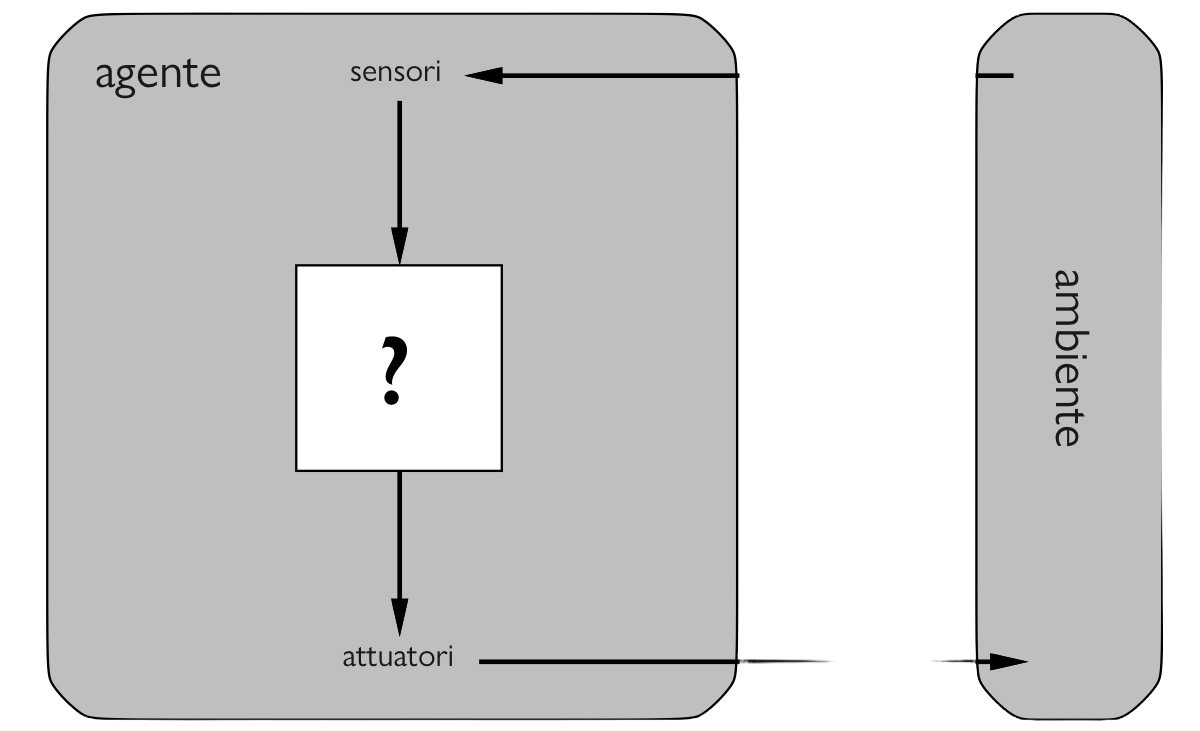
\includegraphics[width=0.4\textwidth, keepaspectratio]{foto/agente-ambiente.png}
      \caption{agente razionale}
    \end{figure}

    Useremo il termine \textbf{percezione} per indicare i dati che i sensori di un agente percepiscono.

    La \textbf{seuquenza percettiva} di un agente è la storia completa di tutto ciò che esso ha percepito nella sua esistenza.

    Sèecificando l'azione prescelta dell'agente per ogni possibile sequenza percettiva, abbiamo descritto l'agente in modo completo.

    In termini matematici diciamo, quindi, che il comportamento di un agente è descritto dalla \textbf{funzione agente}, che descrive la corrispondenza tra una qualsiasi sequenza percettiva e una specifica azione:
    \begin{equation*}
      f : \mathcal{P}^{*} \rightarrow \mathcal{A}
    \end{equation*}

    Possiamo immaginire di rappresentare in forma di tabella la funzione agente che descrive un certo agente.

    Nella maggior parte dei casi questa tabella sarebbe molto grande, di fatto infinito, a meno di non specificare una lunghezza massima delle sequenza percettive che vogliamo prendere in considerazione.

    La tabella è una descrizione esterna dell'agente.

    Internamente, la funzione agente di un agente artificale sarà implementata da un \textbf{programma agente}.

    E' importante tenere distinti questi due concetti:
    \begin{itemize}
      \item \textit{funzione agente}: descrizione matematica stratta
      \item \textit{programma agente}: implemenyazione concreta della funzione agente, in esecuzione all'interno di un sistema fisico.
    \end{itemize}

    \section*{Strategie di ricerca non informata}
    \addcontentsline{toc}{section}{Strategie di ricerca non informata}
    Un \textbf{algoritmo di ricerca non informata} non riceve alcuna informazione su quanto uno stato sia vicino all'obiettivo.

    Es: consideriamo una persona che si trova ad Arad con l'obiettivo di raggiungere Burarest.

    Una persona non informata, priva di conoscenza della geografia romena, non ha modo di sapre se sia meglio come primo passo andare a Zerind o Sibiu.

    \subsection*{Ricerca in ampiezza}
    \addcontentsline{toc}{subsection}{Ricerca in ampiezza}
    Quando tutte le \hl{azioni hanno lo stesso costo}, una strategia appropriata è la \textbf{ricerca in ampiezza}, in cui si espande prima il nodo radice, poi tutti i suoi sucessori, poi i sucessori di quest'ultimi, e così via.

    Potremmo implementare la ricerca in ampiezza, chiamata \textbf{RICERCA-BEST-FIRST}, con la funzione di valutezione $f(n)$ è uguale alla profondità del nodo, cioè al numero di azioni necessario per ragiungerlo.

    Una coda FIFO (First In First Out) risulterà più veloce di una coda con priorità e ci fornirà l'ordine corretto dei nodi: i nuovi nodi vanno in fondo alla coda e quelli vecchi, a profondità minore, vengono espansi per primi.

    Inoltre, raggiunti può essere un insieme di stati, anzichè una corrispondeza da stati a nodi, perchè una volta raggiunto uno stato, non possiamo più trovare un cammino migliore per raggiungerlo.

    LA ricerca in amppiezza trova sempre una soluzione con un numero minimo di azioni, perchè quando genre nodi di profondità $d$, ha già generato tutti i nodi di profondità $d - 1$, perciò se uno di essi fosse una soluzione, sarebbe stato stato trovato.

    Ciò significa che è ottimale rispetto al costo per problemi in cui tutte le azioni hanno lo stesso costo, ma non per problemi che non hanno tale proprietà.

    E' completa in ogni caso.

    In termini di tempo di tempo e spazio, supponiamo di effettuare una ricerca in un albero uniforme dove ogni stato ha $b$ sucessori.

    Allora il numer totale di nodi generati è:
    \begin{equation*}
      1 + b + b^2 + b^3 + \dots + b^d = O(b^d)
    \end{equation*}

    \begin{figure}[H]
      \centering
      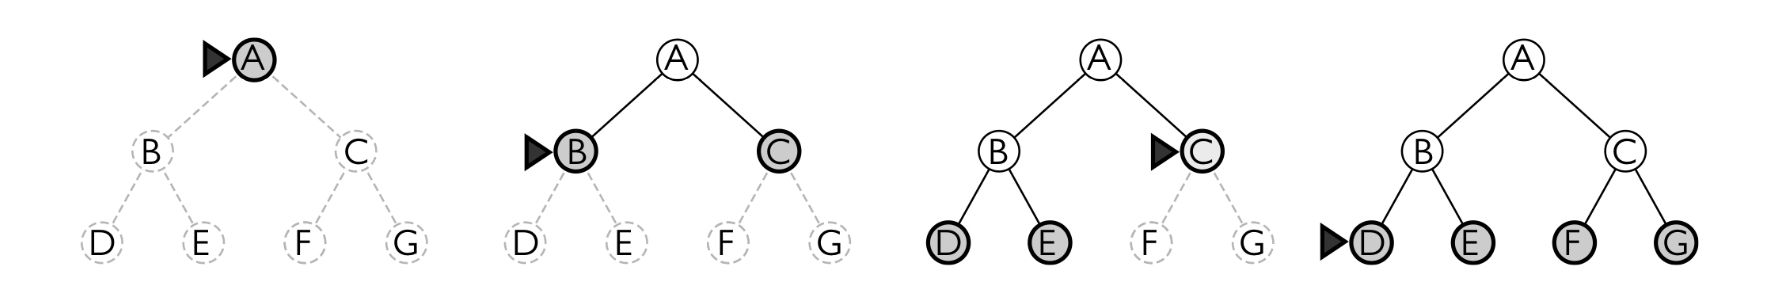
\includegraphics[width=0.7\textwidth, keepaspectratio]{foto/ricercaInAmpiezza.jpeg}
      \caption{algoritmo BFS}
    \end{figure}

    %pseudo-codice algoritmo

    \begin{example}
      \begin{lstlisting}[language=Python, breaklines=true, linewidth=\linewidth]
        function BFS(problem) returns a solution, or failure
          nodo <- nodo(problema.statoIniziale)
      \end{lstlisting}
    \end{example}

    Tutti i nodi rimangono in memoria, perciò le complessità temporale e spaziale sono entrambe $O(b^d)$, quindi, esponenziali.
    
    Nella ricerca in ampiezza, i requisiti di memoria rappresentano un problrma più importante rispetto al tempo di esucuzione.

    Tuttavia, il tempo rimane comunque un fattore importante.

    In generale, i problemi di ricerca con complessità esponenziale non possono essere risolti mediante ricercche non informate, se non nelle istante più pisccole.

    \subsection*{Ricerca a costo minimo (algoritmo Dijkstra)}
    \addcontentsline{toc}{subsection}{Ricerca a costo minimo (algoritmo Dijkstra)}
    Quando le azioni hanno costi diversi, si utilizza BFS in cui la funzione di valutazione è il costo del cammino della radice al nodo corrente: si tratta dell'\textbf{algoritmo di Dijkstra} o \textbf{ricerca a costo uniforme}.
\end{document}